\documentclass[a4paper, 12pt]{article}

\usepackage{a4}
\usepackage[utf8]{inputenc}
\usepackage[french]{babel}
\usepackage[T1]{fontenc}
\usepackage{graphicx}
\usepackage{amssymb}
\usepackage{listings}
\usepackage{float}
\usepackage{listing}
\usepackage{xcolor} 
\usepackage{mdframed}
\usepackage{enumitem}


\DeclareUnicodeCharacter{2212}{-}
\author{Igor De Bock}
\date{28 décembre 2021}
\title{Git}
\parskip=7pt
\setlength\parindent{0pt}
\lstset{language=sh,basicstyle=\ttfamily}
\definecolor{light-gray}{gray}{0.95}

\begin{document}
    \maketitle
    \tableofcontents

    \section{Introduction}

    Git est un VCS ; un système de contrôle des versions. Un logiciel de
    contrôle des versions traque les modifications apportées à un projet
    (dossier) pour qu'on puisse retourner à une version spécifique. Plus
    généralement, ce type de programmes offre des fonctionnalités pour facilité
    le développement.

    \section{Concepts}

    \subsection{Snapshots}

    Généralement, un VCS traque le progrès sous la forme d'une liste de
    changements effectués sur les fichiers du dossiers. Chaque changement est
    appelé \textit{delta} ($\Delta$), c'est pourquoi ces VCS sont dit de type 
    \textit{delta-based}.

    \begin{figure}[H]
        \centering
        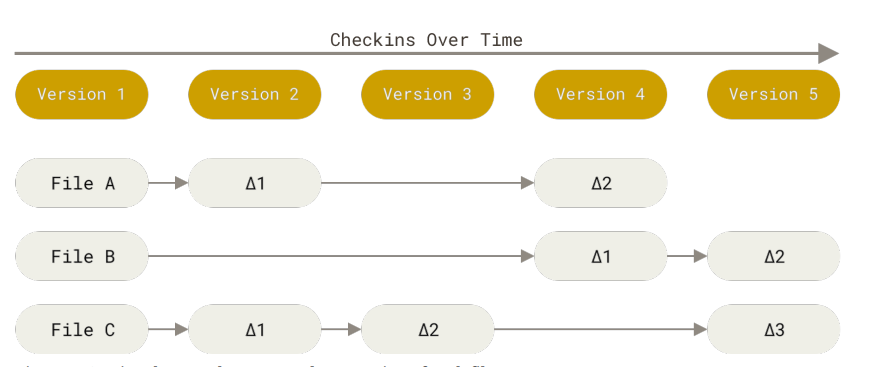
\includegraphics[scale=0.54]{figs/delta_based_cvs.png}
        \caption{Suivit du progrès sous la forme de \emph{deltas}}
        \label{fig:graphcommit}
    \end{figure}

    Une des caractéristique principales de git est qu'il n'utilise pas le
    système de deltas, mais un système de \emph{\textit{snapshots}}.

    Un snapshot est copie du contenu du dossier/projet. On peut se représenter
    un snapshot comme une photo/image du projet. Git nous permet essentiellement
    de prendre un snapshot de la version actuelle du projet et de l'ajouter à
    la fin d'une chaine contenant toutes les snapshots pris précédemment. Git
    traque donc le changement par le biais d'une longue chaine contenant, de
    manière chronologique, les snapshots/versions/copies du projet.

    Git, traquant le changement par une série chronologique d'images, on peut
    faire l'analogie de la vidéo.  Toutefois, on ne prend pas 24 snapshots par
    secondes. Généralement, on en prend qu'un après avoir fini une \textit{unité
    de travaille}, càd fixé un bug, ajouté une fonctionnalité etc.

    \begin{figure}[H]
        \centering
        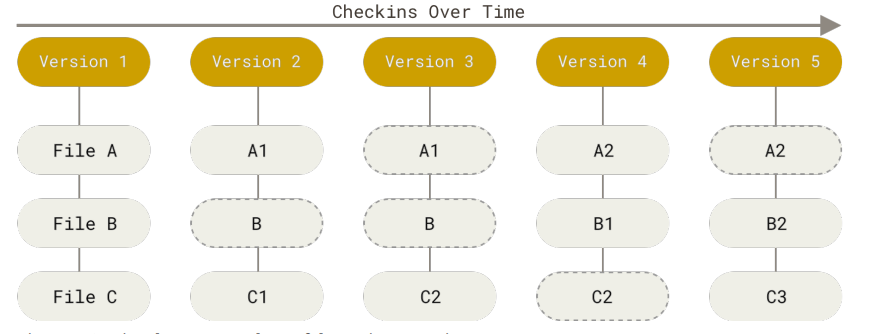
\includegraphics[scale=0.54]{figs/snapshot_based_cvs.png}
        \caption{Suivit du progrès sous la forme d'une série de snaphots (ici
        chaque snaphot correspond à une version)}
        \label{fig:graphcommit}
    \end{figure}

    Comme on le constate  sur cette figure, git ne restocke pas les fichiers
    inchangés. Pour des raisons d'éfficacité, il stocke juste un lien vers le
    fichier du snapshot précédent (pour plus de détails sur le fonctionnement,
    voire la section \ref{ss:commithist})

    \subsection{Branches}
    
    Git supporte les ramifications/branches et leur fusion. Une branche est
    une copie du projet, une nouvelle ligne de développement/chaine de
    snapshots qui diverge de la chaine principale. 

    Les branches sont un moyen de développer une nouvelle fonctionnalité tout en
    gardant la branche principale fonctionnelle ou sans entraver son
    développement. Une fois la nouvelle fonctionnalité débugger et prête à être
    déployée, on peut fusionner la branche secondaire dans la branche
    principale.

    Par default, un projet n'est fait que d'une chaine qui est appelée master
    ou main. Pour créer des ramifications, voire section \ref{se:commandes}.

    \begin{figure}[H]
        \centering
        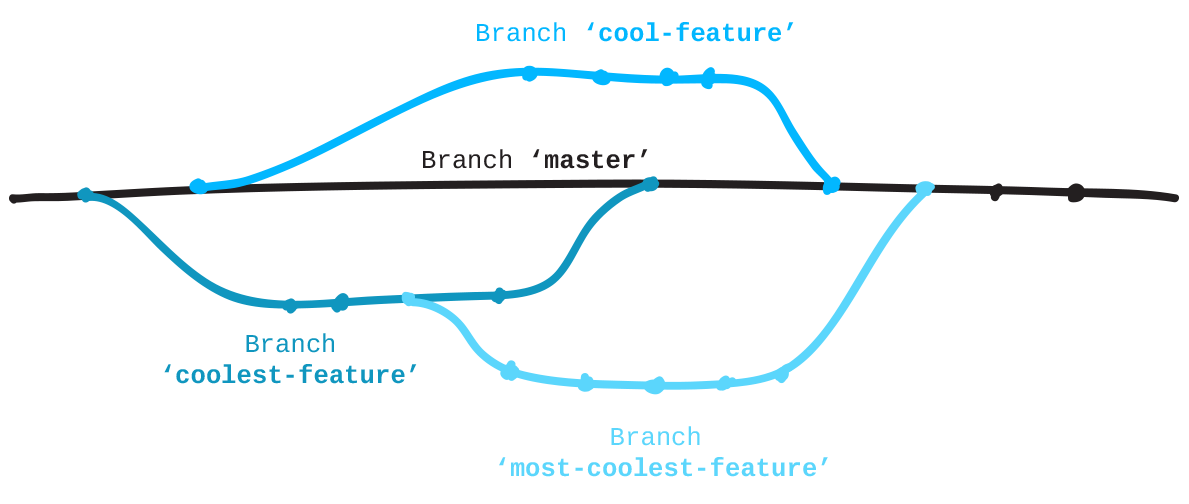
\includegraphics[scale=0.24]{figs/branches.png}
        \caption{Stratégie de developpement simple avec ramifications}
        \label{fig:branches}
    \end{figure}

    Les branches sont souvent utilisées de manières plus poussée comme
    ci-dessous.

    \begin{figure}[H]
        \centering
        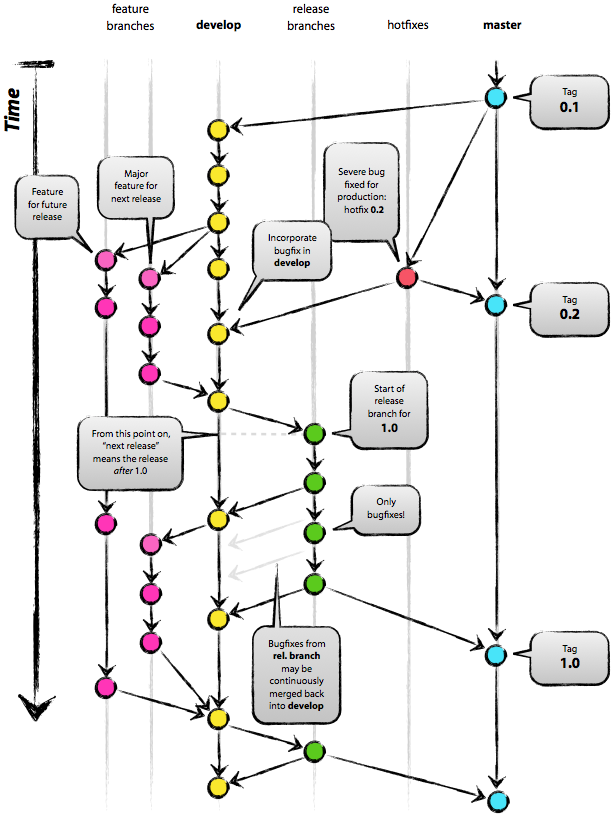
\includegraphics[width=0.6\textwidth]{figs/branches_complicated.png}
        \caption{Stratégie de developpement complexe}
        \label{fig:branchescomp}
    \end{figure}
    
    \subsection{Remotes}

    Un remote est un dépôt (voire \ref{s:dépôt}) qui tracke le même projet mais
    qui réside autre part. Généralement, un projet a un remote hébergé en ligne
    (sur une platforme comme Github ou Gitlab) qui permet la collaboration.
    Chaque personne à sa version du projet sur son ordinateur, mais toute
    l'équipe partage le remote. Une fois qu'un membre a apporté des
    modifications à sa version locale, il peut les incorporer/publier dans le
    remote pour que les autres puisse mettre les télécharger et mettre à jours
    leur version.

    \begin{figure}[H]
        \centering
        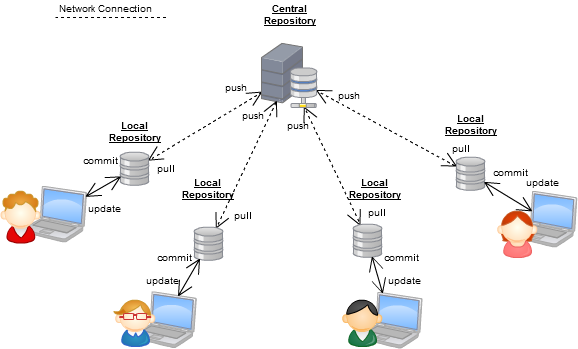
\includegraphics[width=0.7\textwidth]{figs/remotes.png}
        \caption{Collaboration avec remote repository}
        \label{fig:remotes}
    \end{figure}

    Dans ces relations entre dépôt, les dépôts locaux sont appelés les dépôts
    downstream, alors que le remote, le dépôt central, est appelé le dépôt 
    upstream.

    \subsection{Les tags}
    Comme la pluspart des VCS, git permet de "tagger", donner une étiquette à
    un point considéré comme important. Généralement, on utilise cette
    fonctionnalité pour marquer les états de publicatoins (avec les étiquettes
    v1.0, v1.1 et ainsi de suite).  Les tags sont aussi souvent utilisés pour
    créer des points de restaurations.

    \begin{figure}[H]
        \centering
        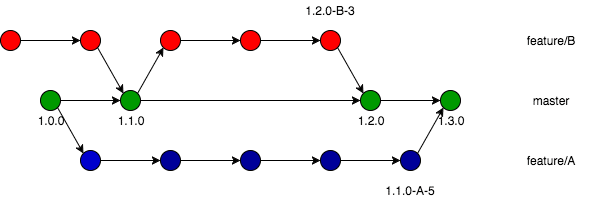
\includegraphics[width=1\textwidth]{figs/tags.png}
        \caption{Etiquetage de commits}
        \label{fig:tags}
    \end{figure}
        
    
    \section{Le dépôt et fonctionnement de git}\label{s:dépôt}
    \subsection{Dépôt et working directory}
    Un projet sous git est entièrement contenu dans un \emph{dépôt git}. Le
    dépôt git est une base de donnée contenant toutes les informations du
    projet (la liste des snapshots et leur contenu, les branches, les paramètres
    etc). Celui-ci est contenu dans un dossier nommé \textit{.git}.

    Ce dossier, étant une \textit{data-structure}, stocke le contenu du dépôt de
    manière éfficace, mais est très difficile à comprendre et utiliser
    "manuellement". Git est en quelque sorte un programme qui fait
    l'intermédiaire entre un dépôt git et l'humain ; qui nous permet d'interagir
    (lire, modifier,...) avec cette base de donnée.

    Pour ce faire, git offre des commandes et le \textit{working directory}.
    Le working directory est le dossier dans lequel se trouve le dépôt/dossier
    .git. Git va essentielement y décompresser le contenu du dernier snapshot
    (plus précisemment le snapshot \textit{HEAD}, voire section
    \ref{sss:branches}) dans des fichiers/dossiers réels et ainsi utilisables.
    Le working directory est donc une copie "brute" de la dernière version du
    projet sur laquelle on peut travailler. 

    Une fois qu'on a appliqué des modifications au working directory, on peut
    incorporer les nouvelles versions des fichiers/dossiers dans le 
    dépôt/l'historique des snapshots en passant par le \textit{staging area}.

    Le staging area permet de préparer le prochain snapshot. On y décrit les
    modifications qui devront apparaîtres dans le prochain commit. Pour plus
    d'informations sur le staging area, voire \ref{ss:stagingarea}
    
    \begin{figure}[H]
        \centering
        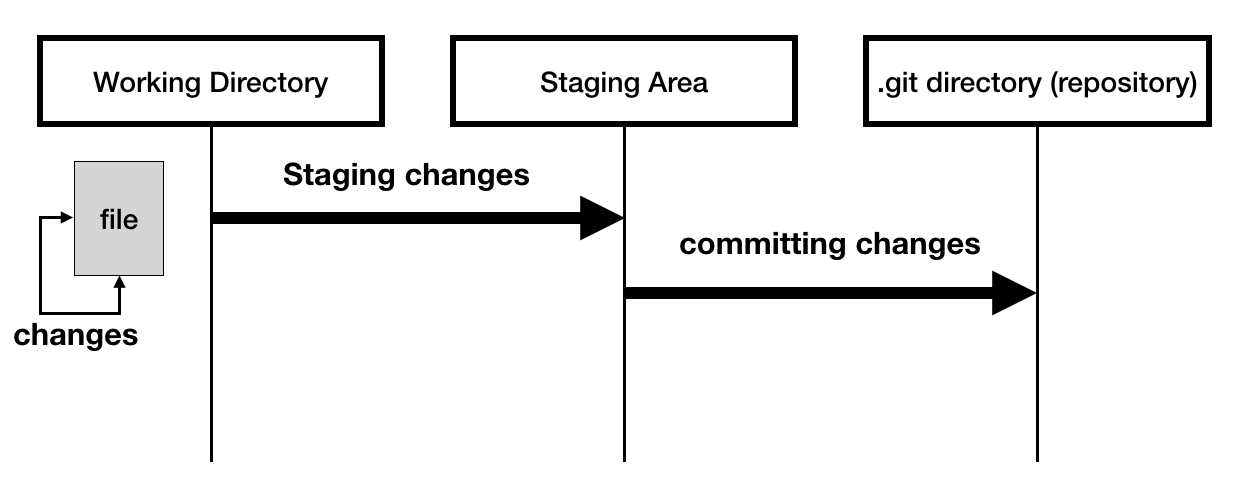
\includegraphics[width=0.9\textwidth]{figs/three_areas.png}
        \caption{La relation entre le working directory, le staging area et le
        dépôt git.}
        \label{fig:3areas}
    \end{figure}

    %branches très légère.
    \subsection{Les deux datastructures majeures}
    Un dépôt git est prinipalement constitué de deux datastructures, une base de
    donnée d'objet immuables pour stocker la chaine de snasphots, et un index
    mutable qui garde le staging area.

    \subsubsection{La base de donnée d'objets}
    La base de donnée d'objets est utilisée pour stocker la chaine de snapshots
    et ses ramifications. Elle est constituée de trois types d'objets :
    \begin{itemize}
        \item les BLOBS ;
        \item les trees ;
        \item les commits.
    \end{itemize}

    Ces objets sont simplement des fichiers qui sont contenus dans le dossier
    \textit{./.git/objects}. Les objets sont identifiés/nommés par leur hash et
    se référence entre eux par celui-ci

    L'objet blob est utilisé pour décrire un fichier. C'est une copie conforme
    d'un fichier du projet, à l'exeption qu'il ne contient aucune métadonnée.
    Il ne contient que le contenu d'un fichier, pas de date de création,
    d'auteur etc. 

    L'objet tree est utilisé pour décrire un dossier. Un objet tree est une
    liste des identifiants (hash) des blobs et des trees correspondant
    aux fichiers et sous-dossiers contenu dans le dossier qu'il décris. Un objet
    tree contient aussi les six premiers caractères de l'objet tree parent.
    Les objets tree qui n'ont pas de tree parent sont appelés "root" et
    représente un snaphshot.

    \begin{figure}[H]
        \centering
        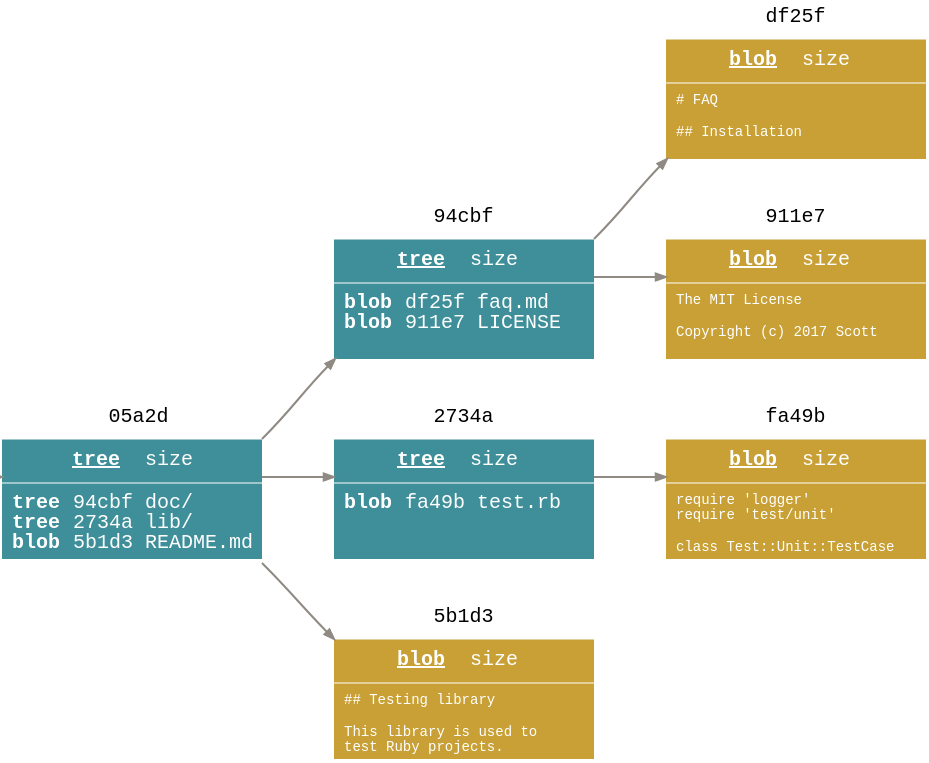
\includegraphics[width=0.8\textwidth]{figs/tree_object.png}
        \caption{Représentation d'un tree root}
        \label{fig:tree}
    \end{figure}

    L'objet commit va contenir un snapshot. Celui-ci contient un auteur, 
    une description, un timestamp, un hash identifiant, l'indentifiant/hash du
    commit parent (pour définir sa place dans la chaine) et le hash de l'objet
    tree root décrivant le snapshot. 

    \begin{figure}[H]
        \centering
        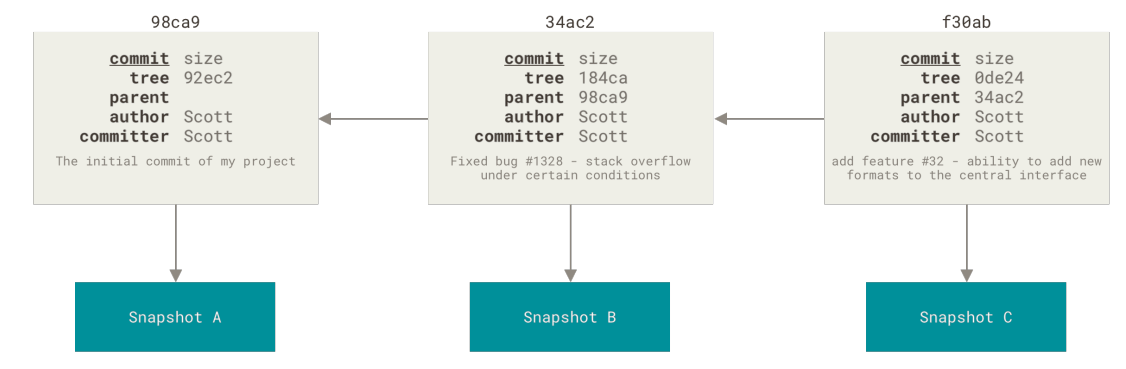
\includegraphics[width=0.9\textwidth]{figs/commits.png}
        \caption{Chaine de commits et leurs contenu.}
        \label{fig:commit}
    \end{figure}

    Une branche est une chaine de commit, une ligne de développement. Ainsi, 
    une branche est définie par son dernier commit. En effet, à partir de
    celui-ci, on peut retracer toute la chaine car chaque commit pointe vers
    celui qui le précède. Git va décrire une branche de cette manière ; par un
    simple pointeur vers un commit. 
    
    Avec git, une branche est donc un objet très léger. Pour ajouter un commit,
    il suffit de l'accrocher au commit référencé par le pointeur et ensuite
    d'avancer le pointeur d'un commit pour qu'il référence la nouveau dernier 
    commit.

    Quand on crée un dépôt, git va créer une branche/pointeur nommée par
    default \emph{master}. A chaque fois qu'on commit, le pointeur avance
    automatiquement.
    
    Quand on crée une nouvelle branche, git crée simplement un nouveau pointeur
    pointant vers le dernier commit. Ce pointeur/branche, étant un ref (voire
    \ref{ss:tagrem}), est contenu dans le fichier \lstinline{refs/heads/master}.
    A ce moment, master et le nouveau pointeur qu'on appellera ici
    \textit{feature} pointe vers le même commit et sont donc identiques. Ceci
    est normale, ils partageronts toujours cette chaine de début, mais à partir
    de maintenant, leurs chaines vont diverger.

    Ceci car, quand on ajoutera un commit à master, master avancera vers le
    nouveau commit mais feature ne bougera pas. Il pointera toujours vers son
    dernier commit. De la même manière, quand on va ajouter un commit à feature,
    git va l'attacher à son dernier commit qui le rappelons est déjà le
    parent d'un commit de master. Ce commit sera donc le parent de deux commit
    et est ainsi le point où les deux chaines divergent. Cette propriété (un
    commit peut avoir plusieurs enfants) permet à la base de donnée d'objet de
    décrire les branches.

    \begin{figure}[H]
        \centering
        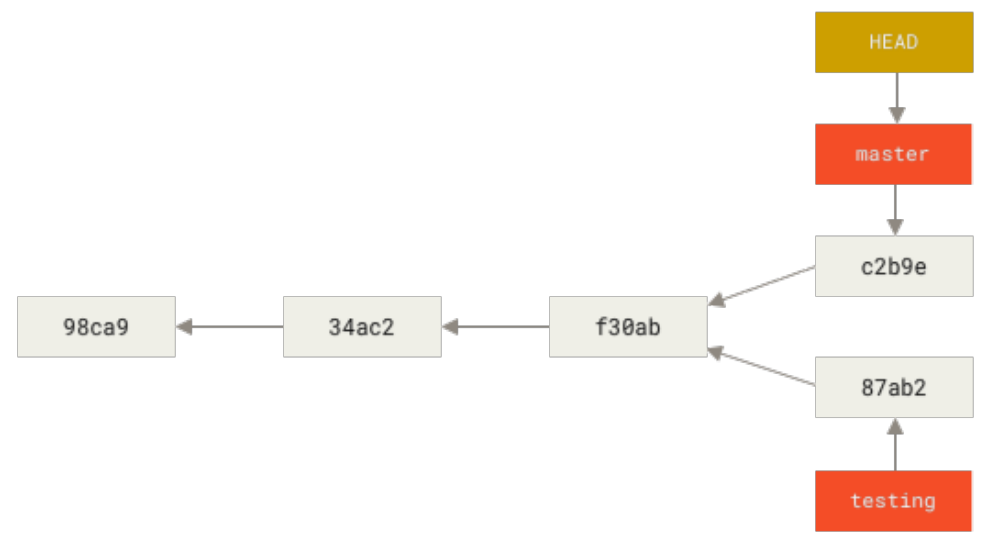
\includegraphics[width=0.9\textwidth]{figs/branches_HEAD.png}
        \caption{Point de divergence de deux branches}
        \label{git:branchdiverg}
    \end{figure}

    Sur cette figure, on peut remarquer l'inscription \textit{HEAD}. HEAD est
    une variable qui contient le pointeur (branche) actif. Un commit est ajouté
    au commit référencé par le pointeur contenu dans HEAD aussi appelé commit
    HEAD. Ainsi, changer de branche est une opération très légère, il suffit de
    changer le pointeur contenu dans HEAD.

    Tout comme un commit peut avoir plusieurs enfants pour lancer une branche,
    un commit peut avoir plusieurs parents et être le point de fucsion de
    deux branches.

    \begin{figure}[H]
        \centering
        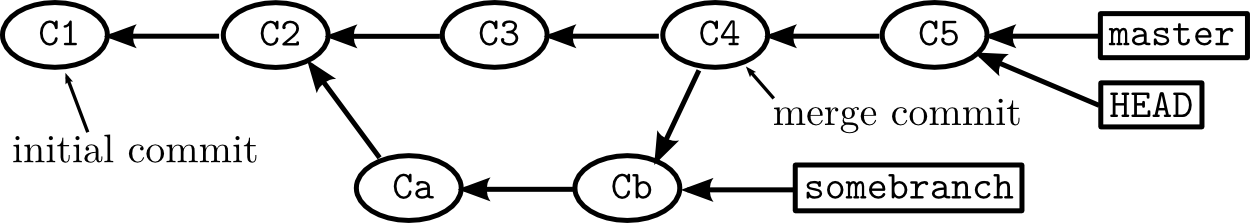
\includegraphics[width=0.9\textwidth]{figs/brancheshistory.png}
        \caption{fusion de branches}
        \label{fig:fusion}
    \end{figure}
    Sur cette figure, les commit \emph{Ca} et \emph{Cb} font aussi partie de la
    branche master. De la même façon, les commits \emph{C1} et \emph{C2}
    appartiennent aussi à branche somebranch. Toutefois, les commits \emph{C4}
    et \emph{C5} n'appartiennet pas à la branche somebranch, la branche
    somebranch étant le commit \emph{Cb} avec tous ceux qui le précèdent.

    Une fusion est un processus très complexe mais peut être réduit à 3 étapes.
    Pour fusionner X et Y, les étapes sont :

    \begin{enumerate}
        \item Trouver une base de fusion entre X et Y. Une base de fusion est
        généralement le dernier commit (vesion) commun aux deux branches. On
        appelera cette version B.
        \item Effectuer les \textit{diffs} de X avec B et de Y avec B. Faire un
        diffs signifie d'executer un programme de comparaison des données. Ce
        genre de programmes trouve la plus longue séquence de lignes communes
        (LCS problem) entre deux fichiers, et à partir de celle-ci, détermine
        toutes les différences/modifications par une série de suppression et
        d'insertion de lignes. Git va faire les choses un peu différemment et
        va trouver les insertions/suppressions et les associés à des endroits en
        les comparant avec leur environnements.
        \item Git compare les deux diffs. Si les deux introduisent la même
        modification au même endroit, celle-ci est acceptée ; si l'un introduit 
        une différence et l'autre laisse la régions intact, elle est acceptée ; 
        si les deux introduisent des modifications différentes au même endroit,
        il y a un conflit qu'il faut résoudre manuellement.
        

    \end{enumerate}

    Si on veut fusionner X et Y, git va chercher leur dernier commit
    (version) commun (qui se trouve sur les deux branches). On va appeler cette
    version B. Git va lister les différences qu'il y a entre X et B et Y et B.
    Pour chaque modifications, 
    
    Puis va lister toutes les différences qu'il y a entre X et B et
    Y et B (sous la forme de diffs)  

    \subsubsection{La structure muable}\label{ss:stagingarea}

    La structure muable est, comme dit ci-dessus, utilisée pour stocker l'index 
    plus communément appelée le staging area.

    L'index contient un snapshot muable. Pour ce faire, la datastructure est
    différente. A la place d'utilisé une arborescence d'objet tree, l'index est
    un simple fichier, qui contient une liste de chemin d'accès de fichiers
    chacun associé au hash d'un blob. Le chemin d'accès définis alors la
    place et le nom du fichier tandis que le hash, et par extension, le blob, en
    définis le contenu.

    \begin{figure}[H]
        \centering
        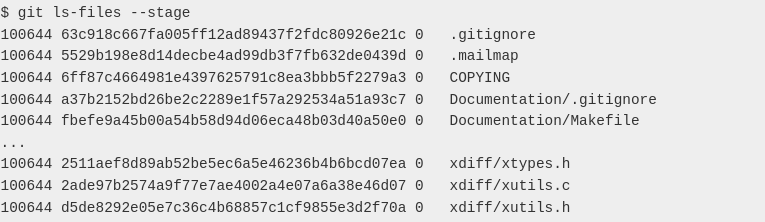
\includegraphics[width=\textwidth,]{figs/index.png}
        \caption{Contenu d'un index décompresser. Les 6 premiers chiffres
        indique les permissions, la séquence suivante est le hash et la dernière
        est le chemin d'accès.}
        \label{fig:index}
    \end{figure}

    Ainsi, cette structure est muable contrairement à l'arborescence, qui, à la
    manière des blockchains est "hashée". Pour modifié le contenu d'un fichier
    du snasphot, il suffit d'ajouter un nouveau blob (dans le dossier
    \lstinline{./.git/objects}) contenant le contenu modifié et de changer le
    hash associé au fichier par celui du nouveau blob. De la même manière, pour
    supprimer ou ajouter un fichier, il suffit de supprimer ou rajouter une
    entrée dans la liste.

    Quand on prend un commit, git capture le snapshot décris par l'index pour
    constuire l'objet tree root imuable ; l'index représente le contenu du
    prochain commit et est en quelque sorte sa zone de préparation. De cette
    manière, l'index fais le liens entre le working directory et la chaine de
    commits, permet d'incorporer des modifications dans la chaine par la manière
    décrite ci-dessus (qui n'est bien sûr pas faite manuelement, voire
    \ref{git:add})


    \subsection{Les remotes} 

    Avec git, un remote est simplement un nom associé à une URL : un alias.
    Généralement, on a qu'un remote qu'on appelle par convention
    \textit{origin}. Si on veut le référencer, on utilise ce nom. Toutefois, on
    peut en avoir autant qu'on veut, et leurs donner n'importe quel nom.

    Deux dépôt communiquent en s'envoyant leurs refs et les objets associés.
    Un ref est un fichier qui contient le hash d'un commit. Ce sont des poiteurs
    vers un commit qui porte le nom du fichier. Un refs stockés dans le dossier
    \lstinline{./.git/refs}. Les branches et les tags sont par exemple des refs.

    Quand on se synchronise à un remote, celui-ci envoit tous ses refs ainsi que
    les objets nécessaires pour complêter leur historique. Ces objets sont
    simplements mis avec les autres (dans \lstinline{./.git/objects}) tandis que
    les refs sont mis dans un nouveau dossier au nom de
    \lstinline{./.git/remotes/<alias-url-remote>} (il y a donc un dossier par
    remote).

    Ce dossier contient donc toutes les branches et les tags du remote. Ces
    branches sont ce qu'on appelle des \textit{remotes tracking branches}. On
    ne peut pas y toucher et elles sont mises à jour à chaque 
    connection/synchronisation avec le remote (par le biais de la commande
    \lstinline{fetch} voire section \ref{se:commandes}). Une remote tracking
    branch prend le nom \lstinline{<alias-remote>/<branch>} et se trouve dans le
    fichier \lstinline{./.git/remotes/<alias-remote>/<branch>}. 

    Une remote tracking branch représente donc localement une branche d'un
    remote et indique à git les différences qu'il y a entre notre dépôt et le
    remote.

    \begin{figure}[H]
        \centering
        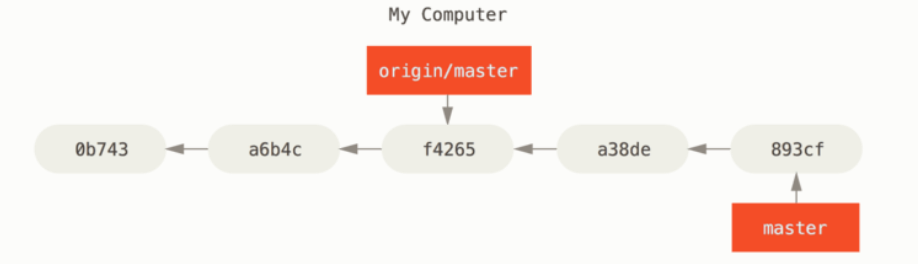
\includegraphics[width=\textwidth,]{figs/remote_tracking_branches.png}
        \caption{Etat du RTB origin/master par rapport à la branche master}
        \label{fig:rtbranches}
    \end{figure}

    Sur cette figure, on remarque qu'on a ajouter deux commits depuis la
    dernière synchronisation avec origin. Qu'on a deux commits
    d'avance/non-synchronisés. De cette manière, git sait qu'à la prochaine
    synchronisation (avec la commande \lstinline{push}), il faut envoyer le
    nouveau ref vers \lstinline{893cf} ainsi que les objets qui font les deux 
    commits d'avance.

    \begin{figure}[H]
        \centering
        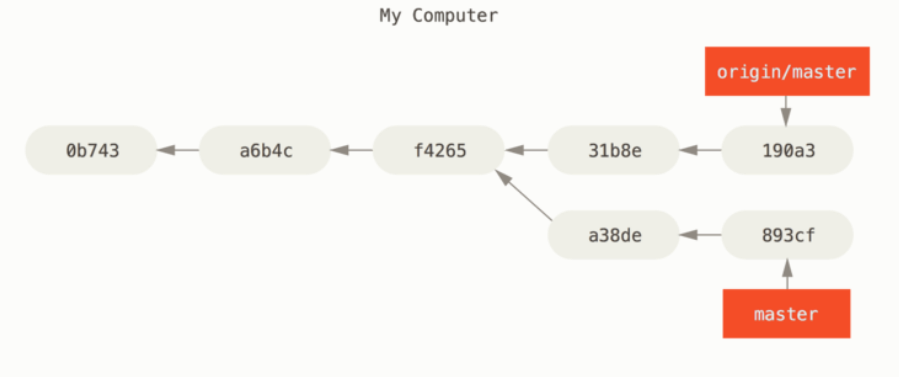
\includegraphics[width=\textwidth,]{figs/fetch.png}
        \caption{Synchronisation des dépôts}
        \label{fig:fetch}
    \end{figure}

    Sur cette image, on a avancé de deux commits, mais le remote à aussi deux 
    commits en plus. Pour intégrés les nouveaux ajouts du remote, il faut
    qu'on fusionne/merge la branche \lstinline{origin/master} dans la branche
    \lstinline{master}.

    Chaque branche locale peut être mise en relation directe avec une remote
    tracking branch. Ceci veut dire que git va prendre conscience de cette
    relation, et va automatiquement traqué les différences entre la branche
    et le remote tracking branche, qui est par extension, la branche upstream
    qu'elle. Git va annoncé combien de commit on a en avance, et les 
    commandes de synchronisation, synchronise par default avec la branche
    upstream mise en relation quand on ne le spécifie pas.

    Quand un branche locale est mise en relation avec une branche upstream, 
    on dit que c'est une \textit{tracking branch} qui traque la branche
    upstream.  

    \section{Commandes}\label{se:commandes}
    \subsection{Clone}
    La commande \lstinline{clone} permet de télécharger un dépôt hébergé en
    ligne (généralement sur github ou gitlab mais peut-être sur un n'importe
    quel ordinateur du réseau).

    Cette commande prend l'URL du dépôt et télécharge le dossier .git qui s'y
    trouve. Une fois le téléchargement terminé, la commande va créer un working
    directory autour du dépôt/dossier .git. Celui-ci portera le nom du dépôt, se
    trouvera dans le repertoire actuelle et sera rempli de la branche/commit
    pointé par la variable HEAD du dépôt en ligne (généralement master ou main).  

    Faire un clone du dépôt officiel de linux : 
    \begin{lstlisting}
    $ git clone https://github.com/torvalds/linux
    \end{lstlisting}

    Par default, git clone va faire de la branche master un tracking branch de
    \lstinline{origin/master}

    Quelques options :
    \begin{description}
        \item[] \lstinline{<directory>} Pour préciser le repertoire dans lequel il
        faut mettre le clone (par default = repertoire actif); 
        \item[] \lstinline{--bare} Indique qu'on souhaite que le dossier .git, et
        qu'il ne faut donc pas créer de working directory ;
        \item[] \lstinline{-n, --no-checkout} Indique qu'il ne faut pas remplir
        le working directory (par la branche HEAD) ;
        \item[] \lstinline{-b <branch>} Pour préciser la branche/le commit vers
        lequel HEAD doit pointé. Comme vu ci-dessus, par default celle-ci
        correspond à la variable HEAD du dépôt en ligne. En conséquence, le
        working directory contiendra cette branche.
    \end{description}
   
    \subsection{Init}
    \lstinline{init} est la seconde commande qui permet de créer un dépôt git.
    Celle-ci crée un sous-dossier .git/dépôt git vide dans le repertoire actif.
    Vide, il ne contient aucun commit et l'index est vierge.

    \noindent Créer un dépôt d'un hypotéthique dossier :
    \lstinline{my_project}.

    \begin{lstlisting}
    $ cd /home/user/my_project
    $ git init
    \end{lstlisting}

    \noindent Créer un dossier à partir de rien :
    \begin{lstlisting}
    $ mkdir new_project
    $ cd new_project
    $ git init new_project
    \end{lstlisting}

    Quelques options :
    \begin{description}
        \item[] \lstinline{<directory>} Si on précise un repertoire, la commande 
        s'execute dans celui-ci ;
        \item[] \lstinline{-b <branch-name>} Pour préciser le nom de la branche
        initiale/principale. Par default celle-ci s'appelle master.
    \end{description}
    \subsection{Config}
    La commande \lstinline{config} permet de configurer git en modifiant le
    fichier \lstinline{./.git/config}.

    \begin{lstlisting}
    # definir le nom d'utilisateur (pour auteur commit)
    $ git config user.name "Igor"
    
    # definir l'adresse email
    $ git config user.email igor.debock@gmail.com

    # definir l'editeur a utiliser
    $ git config core.editor vim

    # definir de la branche par default
    $ git config init.defaultBranch main

    # lister mes parametres 
    $ git config --list
    \end{lstlisting}

    Pour chaqu'une de ces commandes, on peut rajouter le tag
    \lstinline{--global} pour que ces paramètres s'applique sur tous les
    dépôts de l'ordinateur et non celui qui est actif.

    \subsection{Add}\label{git:add}

    La commande \lstinline{add} permet de préparer le prochain commit et va
    ajouter les modifications d'un fichier au staging area.

    \lstinline{add} prend un fichier du working directory, ajoute un blob le
    représentant dans le repertoire \lstinline{./.git/objects}, et va associé ce
    blob au fichier correspondant dans l'index. Plus précisemment,
    \lstinline{add} remplace le hash de l'entrée ayant un chemin d'accès
    correspondant au fichier du workdir par celui du nouveau blob, et de cette
    manière, ajoute des modifications à commit (pour comprendre la démarche,
    voire la section \ref{ss:stagingarea}).

    \noindent Synthaxe :
    \begin{lstlisting}
    $ git add file_to_stage
    \end{lstlisting}

    \noindent \lstinline{add} supporte n'importe quel type de chemins d'accès et
    va agir récursivement sur ceux décrivant plusieurs fichiers :

    \begin{lstlisting}
    # ajouter recursivement un dossier :
    $ git add dossier_a_stage

    # ajouter recursivement tous les pdf : 
    $ git add *.pdf
    \end{lstlisting} 

    \noindent On peut aussi indexer l'entierté du projet avec la commande
    \begin{lstlisting}
    $ git add . # Ici, . represente le dossier root.
    \end{lstlisting}

    Quand on ajoute des fichiers recursivement, tous les fichiers décris dans
    le fichier  \lstinline{./.gitignore} seront automatiquement ignorés, pas
    ajouter. Ceci ne veut pas dire qu'il seront supprimer de l'index et des
    prochains commits, ils seront simplement plus mis à jours car
    \lstinline{add} ne s'appliquera pas sur eux. 

    Quelques options :
    \begin{description}
        \item[] \lstinline{-f, --force} Pour qu'\lstinline{add} ajoute aussi les
        fichiers ignorés (dans \lstinline{./.gitignore})
        \item[] \lstinline{-i, --interactive} Permet d'ajouter interactivement
        le contenu à l'index. 
        \item[] \lstinline{-e, --edit} Ouvre le diff entre les nouveaux blob et
        ancien dans un éditeur et permet de les modifiés. Le but est qu'on
        puisse décider qu'elles lignes doivent êtres ajoutées.
        \item[] \lstinline{-u, --update} Met à jour uniquement l'index pour
        qu'il correspondent au fichiers du working tree. Supprime et modifie
        uniquement les entrées, n'ajoute pas de nouveaux fichiers.  Si avec
        cette option, aucun fichier n'est précisé, (\lstinline{git add -u}),
        applique la commande sur l'entierté du working directory.
        \item[] \lstinline{-A, --all} Ajoute, modifie et supprime les entrées 
        pour que l'index correspondent au working tree. Similaire à
        \lstinline{git add .} à la nuance que ce dernier ne s'applique que sur
        le repertoire actif et est donc similaire si appliqué dans le repertoire
        root.
    \end{description}

    \lstinline{Add} compare des fichiers/dossiers existant dans le working
    directory à l'index. \lstinline{Add} peut donc remarquer des suppressions en
    comparant un dossier, ce qui est par exemple fait avec les commandes
    \lstinline{git add .}, \lstinline{git add -A}, \lstinline{git add -u} ou
    \lstinline{git add <dossier>}. Toutefois, \lstinline{add} ne peut pas
    supprimer un fichier spécifique à cause de cette propriété.
    \lstinline{git add <fichier_supprimer>} ne fonctionne pas. 
    
    Pour supprimer un fichier de l'index, il faut utiliser la commande
    \lstinline{rm}.

    \begin{lstlisting}
    $ git rm <fichier>
    \end{lstlisting}

    Va supprimer l'entrée correspondant à ce fichier dans l'index ainsi que
    le fichier du working directory s'il existe encore. Alternativement

    \begin{lstlisting}
    $ git rm --cached <fichier>
    \end{lstlisting}
    \noindent supprimer uniquement l'entrée et pas le fichier du working
    directory.

    Suivant la même logique, git \lstinline{add} ne sait pas renommer ou bouger
    un fichier.  Pour ce faire, on utilise la commande \lstinline{mv}.
    
    \begin{lstlisting}
    $ git mv <fichier> <directory>
    \end{lstlisting}
    
    \noindent chande le chemin d'accès associé au fichier dans l'index et bouge 
    le fichier dans le working directory. Avec le tag \lstinline{-f, --force},
    la commande écraserait un fichier se trouvant à <directory>.
    
    \subsection{Commit}
    La commande \lstinline{commit} va accrocher un commit à HEAD dont le
    contenu correspond à l'index.

    \begin{lstlisting}
    $ git commit -m "expliqation du commit"
    \end{lstlisting}

    Quelques options
    \begin{description}
        \item[] \lstinline{-a, --all} Pour ajouter automatiquement les
        modifications à l'index avant le commit. N'ajoute pas les nouveaux
        fichiers. Equivalent à d'abord faire un \lstinline{git add -u} 
        \item[] \lstinline{-p, --p} Pour utiliser l'interface patch qui permet
        de préciser interactivement les changements à commit.
        \item[] \lstinline{--amend} Va ajouter les modifications de l'index au
        dernier commit. Supprime le dernier commit et crée un nouveau qui
        est une combinaison du dernier commit et des modifications apportées à
        l'index. Aussi souvent utiliser pour simplement modifier le message du
        dernier commit \\
        \lstinline{git commit -amend -m "nouveauMessage"}
    \end{description}
    \lstinline{commit} permet plusieurs autres flags qui sont forts spécifiques.
    Pour plus d'informations, utiliser la commande lstinline{man git commit}

    \subsection{Status}
    Indique l'état du working tree. Plus précisemment \lstinline{status} affiche
    les chemins d'accès des fichiers qui
    \begin{enumerate}
        \item ont des différences entre l'index et le commit HEAD (y compris
        ceux qui ne sont pas dans le HEAD et dans l'index).
        \item ont des différences entre l'index et le working directory.
        \item sont \emph{untracked}, càd qui ne sont ni dans l'index, ni
        dans commit HEAD, ni dans \lstinline{./.gitignore}.
    \end{enumerate}

    Les premiers sont ceux qu'on commiterais en exécutant un 
    \lstinline{git commit} ; les deuxièmes et troisièmes sont ceux qu'on
    pourrais commit en executant un \\ 
    \lstinline{git add <file> ; git commit}.
    
    Quelques options :
    \begin{description}
        \item[] \lstinline{-s, --short} Pour que le résultat soit plus court 
        \item[] \lstinline{-v, --verbose} Pour qu'en addition des chemins, git
        retourne les modifications effecutées (similaire à 
        \lstinline{git diff --cached}). Si le tag est spécifié deux fois,
        indique en plus les changements qui n'ont pas encore étés indexés
        (similaire à \lstinline{git diff})
    \end{description}

    \subsection{Diff}
    \lstinline{diff} permet d'afficher les différences entre deux commits, entre
    l'index et le commit HEAD, les différences entre le working directory et
    l'index ou une arborescence, les différences résultant d'un merge, les
    différences entre deux objets blob ou les différences entre deux fichiers
    de l'ordinateur. 

    pas fini
    \subsection{Tag}

    \subsection{Branch}
    La commande \lstinline{branch} est utilisée pour lister, créer et supprimer
    des branches.
    
    Pour crée une branche, on utilise la commande : 
    \begin{lstlisting}
    $ git branch <branchname> [<startpoint>]
    \end{lstlisting}

    Cette commande créer un nouvelle branche nommée \lstinline{<branchname>} qui
    pointe vers le commit \lstinline{<startpoint>}. Ce commit peut être un hash
    ou le nom d'une branche. Si la branche est un remote tracking branch (genre
    "origin/master"), la branche la nouvelle branche la traque automatiquement.

    Si startpoint, n'est pas précisé, git utilise le commit HEAD actuel.
    L'option \lstinline{--no-track} précise qu'on souhaite que la branche ne
    traque pas.

    L'option \lstinline{-u} permet de préciser/modifier quel remote tracking
    branch la branche doit traquer :
    \begin{lstlisting}
    $ git branch -u <upstream-branch> <branch>
    \end{lstlisting}
    Ici, \lstinline{<branche>} désigne la tracking branche et
    \lstinline{<upstream-branch>} la branche traquée. Celle-ci est quasiment
    toujours une remote trakcing branch comme \lstinline{origin/master} mais
    peut être n'importe laquelle.

    Pour supprimer une branche, utiliser la commande avec l'option 
    \lstinline{-d, -D}
    \begin{lstlisting}
    $ git branch -d <branchname>
    \end{lstlisting}

    Pour renommer une branche, utiliser l'option \lstinline{-m, -M}
    \begin{lstlisting}
    $ git branch -m <oldbranch> <newbranch>

    # Pour ecraser si <newbranch> existe deja
    $ git branch -M <oldbranch> <newbranch>
    \end{lstlisting}

    Pour lister les branches, utiliser \lstinline{--list}
    \begin{lstlisting}
    $ git branch --list [<pattern>]
    \end{lstlisting}
    Cette dernière utilisation supporte énormemant de paramètres qu'on peut
    trouver dans le manuel.

    \subsection{Checkout}
    \lstinline{checkout} permet de switcher de branche ou de rétablir le
    working directory. Permet en générale de déterminer sur quelle révision on
    veut travailler et réforme le workdir  et l'index en conséquence.

    Pour switcher vers la branche \lstinline{<branch>}, utiliser :
    \begin{lstlisting}
    $ git checkout [<branch>]
    \end{lstlisting}
    La commande va non seulement mettre à jour HEAD, mais va aussi mettre à jour
    l'index et le working directory pour qu'ils correspondent à la branche.

    Si \lstinline{<branch>} est omis (\lstinline{git checkout}), git fais un
    "checkout" de la branche active.  Git restaure, le workdir et l'index
    et les fait correspondre au commit HEAD.

    Pour uniquement restauré un fichier et non l'entierté du workdir, on peut
    utiliser 

    \begin{lstlisting}
    $ git checkout -- <chemin-du-fichier>
    \end{lstlisting}
    Ici les tirets sont facultatifs mais précisent qu'on parle de fichier et non
    pas un paramètre.

    HEAD référence normalement une branche mais peut aussi directement
    référencer un commit. Dans ce cas on est en mode \textit{DETACHED HEAD}, 
    HEAD est dit détaché.
    Pour ce faire, on peut utiliser la commande.

    \begin{lstlisting}
    $ git checkout [--detach] <commit-hash>
    \end{lstlisting}

    Elle nous fais entré en mode DETACHED HEAD sur le commit référencé par
    <commit-hash>. L'index ainsi que le workdir sont mis à jour pour 
    correspondre à celui-ci.

    En mode DETACHED HEAD on n'est pas sur une branche mais sur un commit.
    En conséquence, des nouveaux commits seront accrochés au commit HEAD mais
    vu qu'ils n'appartiendront pas à la branche du commit et que surtout il n'y
    a pas moyen de réecrire l'hitorique, ils divergeront de la chaine sur
    laquelle est le commit dans le vide ou sur ce qu'on peut se représenter
    comme une branche sans nom. Ce genre de commit, détachés de toute branche
    sont appelés DETACHED commit. 

    Entrer en mode DETACHED HEAD est le plus souvent utiliser pour retrouver
    des fichiers, ou juste voir le contenu d'un ancien commit. Des DETACHED
    commits sont aussi utilisés pour faire des expérimentations. Une fois fini
    on peut soit quitter le mode en allant sur un vrai branche
    avec \\
    \lstinline{git checkout <branche/autre commit>} (ce qui supprimera la
    "branche" detachée après un petit temps), ou en faire une vrai branche avec
    \lstinline{git branch <nom>} (ce qui ajoutera un pointeur) qu'on peut par
    après fusionner dans une autre.

    Pour détacher le HEAD au bout d'une branche, utiliser
    \begin{lstlisting}
    $ git checkout <branch> --detach
    \end{lstlisting}

    Pour détacher le HEAD actuelle, càd entrer en mode detached HEAD sur le
    commit actif, on peut plus simplement utiliser
    \begin{lstlisting}
    $ git checkout --detach
    \end{lstlisting}

    \subsection{Remote}
    
    La commande \lstinline{remote} gère l'ensemble des dépôts en ligne.  C'est
    l'intergace qui permet de gérer la liste des entrée de dépôts en ligne qui
    se trouve dans le fichier \lstinline{./.git/config}.

    Pour lister les "remotes", utiliser 
    \begin{lstlisting}
    $ git remote [-v, --verbose]
    \end{lstlisting}
    Avec l'option \lstinline{-v} la commande retourne aussi les urls des
    remotes. 

    Pour ajouter le remote à l'url \lstinline{<url>} et lui donner le nom 
    \lstinline{<name>}, utiliser :
    \begin{lstlisting}
    $ git remote add <name> <url>
    \end{lstlisting}
    Généralement, on utilise le nom \lstinline{origin} pour le remote principal.
    Cette convention vient de git clone. Quand on fait un 
    \lstinline{git clone <url>}, par default, git va ajouter le remote à l'url
    et lui donner le nom \lstinline{origin}. 

    On peut préciser les branches que l'on souhaite du remote et qui devront
    être téléchargée et apparaître dans \lstinline{./.git/refs/remote/} (change
    le refspec) 
    \begin{lstlisting}
    $ git remote add -t <branch> <name> <url>
    \end{lstlisting}

    Pour supprimer la branche \lstinline{<name>} :
    \begin{lstlisting}
    $ git remote remove <name>
    \end{lstlisting}

    Pour renomer la branche \lstinline{<old>} en \lstinline{<new>} :
    \begin{lstlisting}
    $ git remote rename <old> <new>
    \end{lstlisting}

    Pour modifié la liste des branches qui devront être téléchargées.
    \begin{lstlisting}
    $ git remote set-branches <name> <branch1> <b2>...
    \end{lstlisting}
    Avec l'option \lstinline{--add}, la commande ajoute les branches qui suivent
    à la place d'en faire la nouvelle liste.

    Pour récupérer l'url de la branche <name> :
    \begin{lstlisting}
    $ git remote get-url <name>
    \end{lstlisting}

    Pour récupérer des informations sur le remote : 
    \begin{lstlisting}
    $ git branch show <nom-branche>
    \end{lstlisting}
    

    \subsection{Fetch}
    La commande \lstinline{fetch} télécharge les refs (branches et tags) d'un
    remote (les refs précisés dans le refspec) avec les objets nécessaires à
    les complêter.

    On peut voir l'effet de Fetch sur la figure \ref{fig:fetch}, fetch met
    à jour un remote tracking repository mais ne touche pas à la tracking
    branch. Ainsi, c'est une opération qui ne pose jamais de problèmes et peut
    être utiliser sans modération.

    \begin{lstlisting}
    $ git fetch <remote>
    \end{lstlisting}
    Télécharge et met à jour tous les refs (remote tracking branches et tags) du
    remote \lstinline{<remote>}

    pour mettre à jour une branche spécifique 
    \begin{lstlisting}
    $ git fetch <remote> <branch>
    \end{lstlisting}

    \subsection{Merge}
    La commande \lstinline{merge} fusionne plusieurs chaines de
    commits/historiques dans la branche active.

    Quand une branche est fusionnée dans une autre, elle peut toujours être
    continuée après.
    
    \begin{lstlisting}
    $ 
    \end{lstlisting}

    pas fini
    \subsection{Rebase}
    \subsection{Push}
    % la commande entière git push <remote> <local_ref>:<remote_ref> refspec
    La commande \lstinline{push} met à jour les refs du remote en utilisant les
    refs locaux. Avant de push, il faut être sûr que le dépôt local soit à jour
    par rapport au remote avec un \lstinline{fetch} puis \lstinline{merge} car
    git n'accepte pas le push si ce n'est pas un \textit{fast forward merge}.

    \begin{lstlisting}
    $ git push <remote> <branch>
    \end{lstlisting}
     
    Pousse la branche \lstinline{<branch>} au remote \lstinline{<remote>}.

    En ommetant les deux paramètres, git pousse la branche active vers la
    branche traquée si elle porte le même nom.

    \begin{lstlisting}
    $ git push
    \end{lstlisting}

    Quelques options
    \begin{description}
        \item[] \lstinline{-u} Va mettre la branche vers laquelle on pousse
        comme \textit{upstream} de la branche active.
        \item[] \lstinline{--all} Pousse toutes les branches.
    \end{description}

    Les changements 

    pas fini
    \subsection{Pull}
    %expliquer problème branches
    \subsection{Reset}
    pas fini
    \subsection{Log}
\end{document}